%%%%%%%%%%%%%%%%%%%%%%%%%%%%%%%%%%%%%%%%%
% Template LaTeX Template Version 1.0 (December 8 2014)
%
% This template has been downloaded from: http://www.LaTeXTemplates.com
%
% Original author: Brandon Fryslie With extensive modifications by: Vel
% (vel@latextemplates.com)
%
% License: CC BY-NC-SA 3.0 (http://creativecommons.org/licenses/by-nc-sa/3.0/)
%
% Authors: Sabbir Ahmed
% 
%%%%%%%%%%%%%%%%%%%%%%%%%%%%%%%%%%%%%%%%%

\documentclass[paper=usletter, fontsize=12pt]{article}
%%%%%%%%%%%%%%%%%%%%%%%%%%%%%%%%%%%%%%%%%
% Contract Structural Definitions File Version 1.0 (December 8 2014)
%
% Created by: Vel (vel@latextemplates.com)
% 
% This file has been downloaded from: http://www.LaTeXTemplates.com
%
% License: CC BY-NC-SA 3.0 (http://creativecommons.org/licenses/by-nc-sa/3.0/)
%
%%%%%%%%%%%%%%%%%%%%%%%%%%%%%%%%%%%%%%%%%

\usepackage{geometry} % Required to modify the page layout
\usepackage{multicol}
\usepackage{amsmath}
\usepackage{amssymb}

\usepackage[pdftex]{graphicx}
\usepackage{wrapfig}
\usepackage[font=scriptsize, labelfont=bf]{caption}
\usepackage[utf8]{inputenc} % Required for including letters with accents
\usepackage[T1]{fontenc} % Use 8-bit encoding that has 256 glyphs

\usepackage{avant} % Use the Avantgarde font for headings
\usepackage{courier}
\usepackage{xparse}
\usepackage{xcolor}
\usepackage{listings}  % for code verbatim and console outputs

\setlength{\textwidth}{16cm} % Width of the text on the page
\setlength{\textheight}{23cm} % Height of the text on the page
\setlength{\oddsidemargin}{0cm} % Width of the margin - negative to move text left, positive to move it right
\setlength{\topmargin}{-1.25cm} % Reduce the top margin

\setlength{\parindent}{0mm} % Don't indent paragraphs
\setlength{\parskip}{2.5mm} % Whitespace between paragraphs
\renewcommand{\baselinestretch}{1.5}

\definecolor{green}{rgb}{0.18, 0.55, 0.34}

\graphicspath{ {figures/} }
\captionsetup[table]{skip=10pt}

\lstset{language=C, keywordstyle={\bfseries \color{black}}}

% defines algorithm counter for chapter-level
\newcounter{nalg}[section]

%defines appearance of the algorithm counter
\renewcommand{\thenalg}{\thesection .\arabic{nalg}}

% defines a new caption label as Algorithm x.y
\DeclareCaptionLabelFormat{algocaption}{Algorithm \thenalg}

% defines the algorithm listing environment
\lstnewenvironment{pseudocode}[1][] {
    \refstepcounter{nalg}  % increments algorithm number
    \captionsetup{font=normalsize, labelformat=algocaption, labelsep=colon}
    \lstset{
        breaklines=true,
        mathescape=true,
        numbers=left,
        numberstyle=\scriptsize,
        basicstyle=\footnotesize\ttfamily,
        keywordstyle=\color{black}\bfseries,
        keywords={input, output, return, parallel, function, for, to, in, if,
        else, foreach, while, and, or, new, print},
        xleftmargin=.04\textwidth,
        #1
    }
}{}

\renewcommand{\familydefault}{\sfdefault}  % default font for entire document
 % specifies the document layout and style

\begin{document}

    \documentinfo {\textbf{Homework 5: Snake Levels and Obstacles Report}}
    {\today} {Sabbir Ahmed}
    \vspace{-0.1in}

    \section{Background} For this assignment, the previous Snake Game from HW04
    was reimplemented with additional features such as levels and obstacles.

    The game was to conform to the following specifications:

        \begin{itemize}

            \item The obstacles should be drawn in magenta, but otherwise are
            like the fence and the game should stop once the snake (head)
            overlays an obstacle.

            \item The game field should be initiated with no obstacles in the
            field of play for Level 0, and proceed just as in HW4 until the 5th
            apple is eaten.

            \item Every time the player eats 5 apples within a level, a new
            level should be generated with 10 more obstacles than the previous
            level and play should restart on that level.

                \begin{itemize}

                    \item Level 0 has no obstacles, Level 1 has ten obstacles,
                    Level 2 has twenty obstacles, and so on...

                    \item The snake size is reinitialized to 1 to start each
                    level

                \end{itemize}

            \item The level score, and the level should be displayed on the LCD
            display. The display should be as follows:

                \[ \texttt{Lyy} \]

                with \texttt{yy} denoting the current level.

            \item When the game ends, append an \texttt{E} as follows:

                \[ \texttt{LyyE} \]

        \end{itemize}

    \section{Design Approach} Several discrete modules from the previous
    implementation were used in this version. The \texttt{direction},
    \texttt{food\_pos} and \texttt{pacemaker} modules were left unmodified. The
    \texttt{snake\_pos} module was modified to truncate the size of the snake
    from 32 to 5. The \texttt{vga\_layout} module was modified to include the
    new coordinate pairs of the obstacles. The speed-up of the snake feature
    after a certain condition was removed.  Additional submodules:
    \texttt{game\_state} and \texttt{lcd\_driver} were integrated into the
    design.
 
    These submodules were connected using a top level module that may be
    visualized with the schematic diagram configured as a block diagram in
    Figure \ref{fig:schematic}. All the modules implicitly accept clock cycles
    as inputs.

    \begin{figure}[ht]
        \begin{center}
            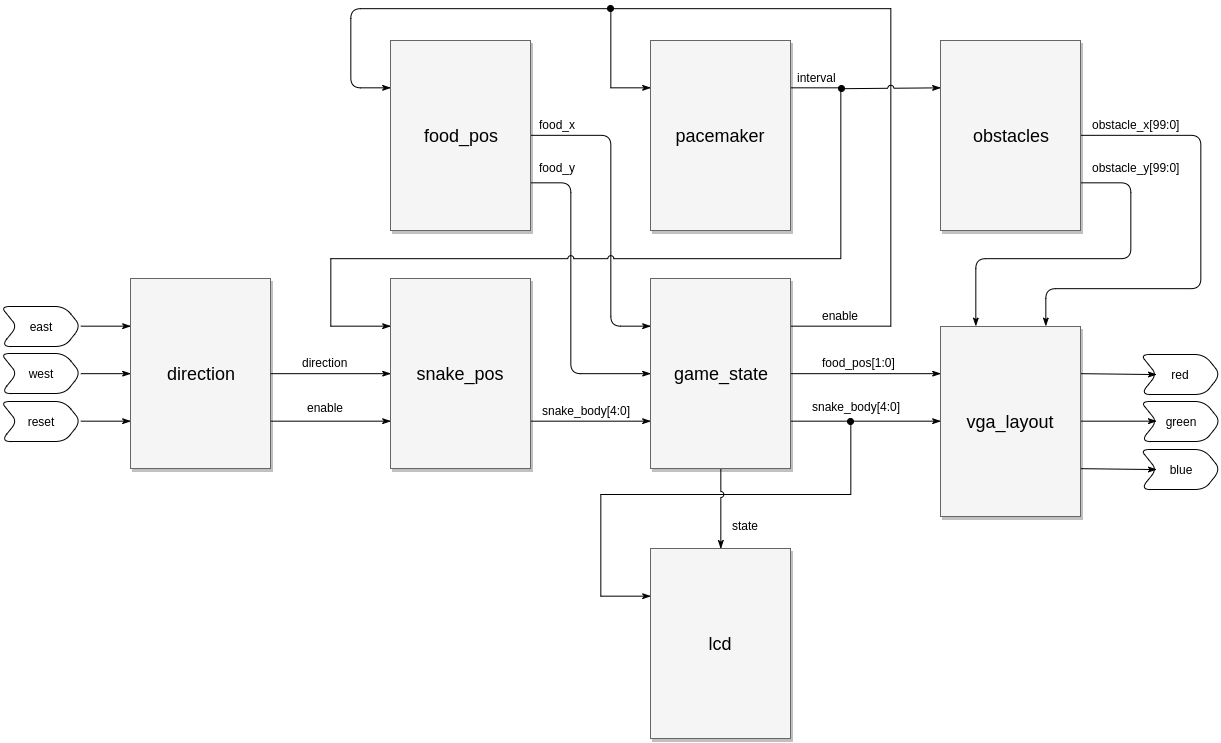
\includegraphics[width=1\textwidth]{top_level_design.png}
            \caption{Block Diagram of the Implementation of the Game}
            \label{fig:schematic}
        \end{center}
    \end{figure}
    \newpage

        \subsection{Direction} The \texttt{direction} module is used to control
        the user inputs. The inputs are one-shotted, debounced and fed into the
        internal state machine to determine the direction the user intended.
        This module sets an enable to the \texttt{snake\_pos} module to notify
        a change in direction.

        \begin{figure}[ht]
            \begin{center}
                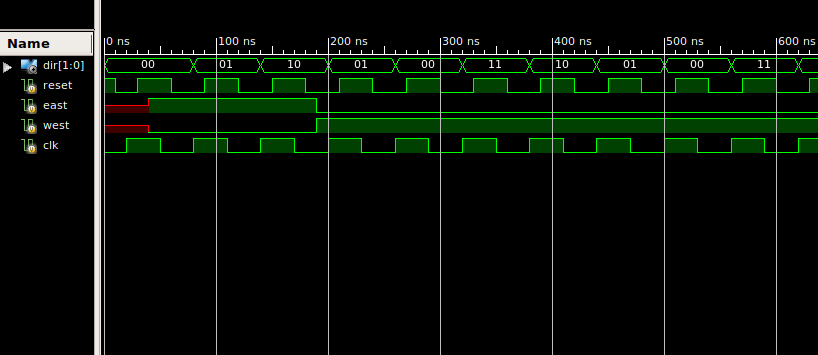
\includegraphics[width=1\textwidth]{direction_wav.png}
                \caption{Waveform of the Testbench of \texttt{direction}}
                \label{fig:direction_wav}
            \end{center}
        \end{figure}

        The sample output demonstrates the \texttt{dir} signal incrementing
        when \texttt{east} is high and decrementing when \texttt{west} is high.

        \subsection{Food} This module generates the \texttt{food\_x} and
        \texttt{food\_y} coordinates of the food when enabled by the
        \texttt{collision} module. The module combinedly utilizes an internal
        counter and a linear feedback shift register to generate the pseudo-
        random coordinates.

        \begin{figure}[ht]
            \begin{center}
                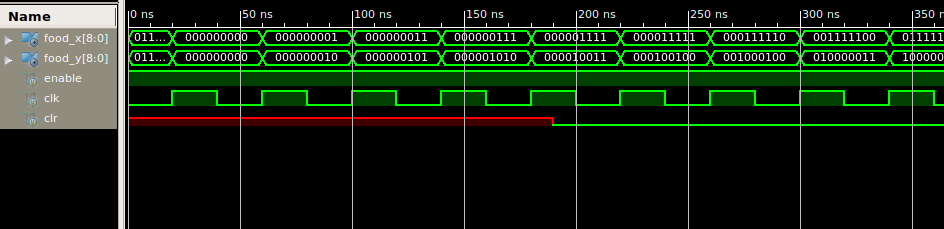
\includegraphics[width=1\textwidth]{food_pos_wav.png}
                \caption{Waveform of the Testbench of \texttt{food\_pos}}
                \label{fig:food_pos_wav}
            \end{center}
        \end{figure}

        The sample output demonstrates the seemingly random coordinates
        generated for \texttt{food\_x} and \texttt{food\_y}.

        \subsection{Snake Segments} The \texttt{snake\_pos} module generates
        the coordinates for the 5 segments of the snake body, including its
        head. The module takes in the 2 bit \texttt{dir} input from
        \texttt{direction} and 2 1-bit control signals from
        \texttt{game\_state}.

        The control signals, \texttt{grow} and
        \texttt{die} are used to indicate the state of the snake body. 

        \begin{itemize}

            \item If both \texttt{grow} and \texttt{die} are disabled, the
            module utilizes \texttt{dir} to shift the body segments.

            \item If \texttt{grow} is enabled and \texttt{die} is disabled, the
            module decrements its internal masking register to enable an extra
            snake segment. The snake segments do not move when they grow.

            \item If \texttt{die} is enabled, the body segments freeze to
            indicate end of the game.

        \end{itemize}

        \begin{figure}[ht]
            \begin{center}
                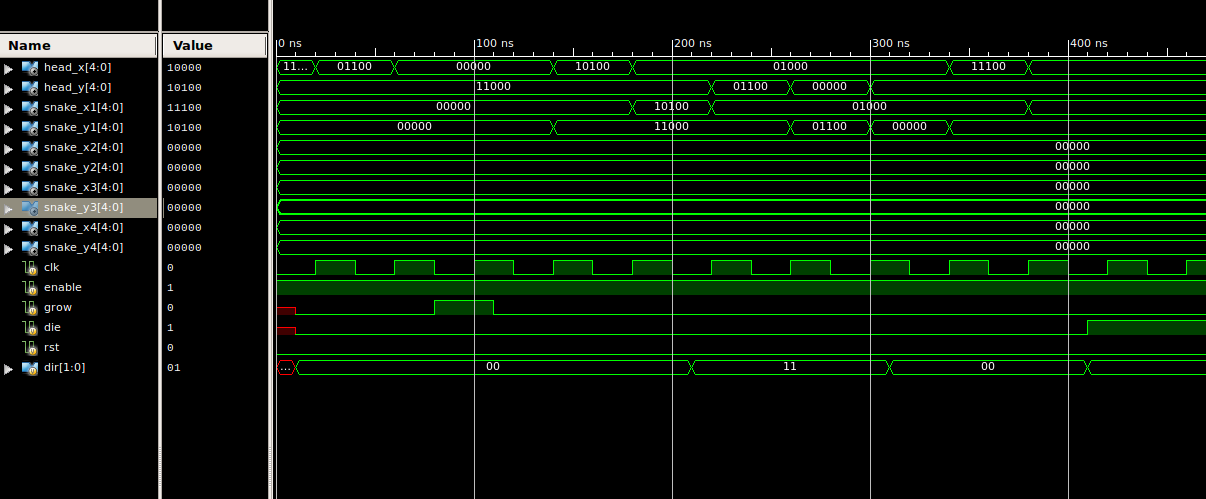
\includegraphics[width=1\textwidth]{snake_pos_wav.png}
                \caption{Waveform of the Testbench of \texttt{snake\_pos}}
                \label{fig:snake_pos_wav}
            \end{center}
        \end{figure}

        The signals were reorganized to highlight the relevant waveforms. The
        sample output demonstrates the movement of the individual body segments
        by utilizing the internal shift register.

        \subsection{Collisions and Levels} The previous \texttt{collision}
        module was integrated into \texttt{game\_state}. The module checks for
        collisions in addition to implementing several of new features. The
        current level of the game is determined by the internal state machine
        of the module. The states proceed to their corresponding next states
        based on serialized checks on collisions with the snake's head with its
        body segments, the fence, and the obstacles per level. Only the third
        and fourth segments are used to check for collisions between the
        snake's head with its body since checking the other segments are
        redundant.

        The module accepts the coordinates of the food and the snake segments
        and determines if a collision has been detected. If a collision has not
        been detected, it sends out an enable signal to the \texttt{snake\_pos}
        module. If a collision with the snake body with the food is detected,
        the internal register \texttt{bite} is incremented. If a collision
        between the snake head and the fence or any of the obstacles is
        detected, the game is frozen.

        The state machine consists of states indicating individual levels of
        the game. Since the game is composed with 3 levels including the zeroth
        level (00, 01, 10, 11), the state machine has 4 states. Each of these
        states generate their corresponding obstacles. The states also
        communicate with the LCD driver to send characters containing the level
        information.

        \subsection{vga\_layout} This module draws the fence of the game, and
        the snake and the randomly placed food on the VGA display. The module
        also uses its input signal \texttt{level} to determine which obstacles
        to display.

        \subsection{Other Modules} Other modules have been provided to be
        utilized for the implementation. \texttt{pacemaker} is used to send out
        enable signals to the other modules such that they update at reasonable
        rates. \texttt{vga\_sync} is used to synchronize the outputs to the VGA
        display. \texttt{lcd\_driver} has been provided to communicate with the
        LCD of the board.

\end{document}
